\documentclass[10pt,twocolumn,letterpaper]{article}

\usepackage{cvpr}
\usepackage{times}
\usepackage{epsfig}
\usepackage{graphicx}
\usepackage{amsmath}
\usepackage{amssymb}

% Include other packages here, before hyperref.

% If you comment hyperref and then uncomment it, you should delete
% egpaper.aux before re-running latex.  (Or just hit 'q' on the first latex
% run, let it finish, and you should be clear).
\usepackage[pagebackref=true,breaklinks=true,letterpaper=true,colorlinks,bookmarks=false]{hyperref}

\cvprfinalcopy % *** Uncomment this line for the final submission

\def\cvprPaperID{****} % *** Enter the CVPR Paper ID here
\def\httilde{\mbox{\tt\raisebox{-.5ex}{\symbol{126}}}}

% Pages are numbered in submission mode, and unnumbered in camera-ready
%\ifcvprfinal\pagestyle{empty}\fi
\begin{document}

%%%%%%%%% TITLE
\title{Cycle-GANs for Cloudy-Sunny Image Translations}
\author{Ayush Baid\\
{\tt\small abaid@gatech.edu}
% For a paper whose authors are all at the same institution,
% omit the following lines up until the closing ``}''.
% Additional authors and addresses can be added with ``\and'',
% just like the second author.
% To save space, use either the email address or home page, not both
\and
Shreya Varshini\\
{\tt\small shreyavarshini@gatech.edu}
\and
Vijay Upadhya\\
{\tt\small vupadhya6@gatech.edu}
}

\maketitle
%\thispagestyle{empty}

%%%%%%%%% ABSTRACT
\begin{abstract}
We studied the task of image-to-image translation, where we learn a mapping function from an input source image to an output photo realistic image that appears to be sampled from the target distribution space, while maintaining similar content to the source image. In this project, we propose image-to-image translation between cloudy and sunny images by employing the cycle consistent generative adversarial learning framework. We start with the baseline architecture and make suitable modifications to the generator and discriminator architectures, coupled with an additional new content similarity objective. We achieve photo realistic image results on a diverse set of input formats. Furthermore, the quantitative evaluation of our generative model gave a reasonable per class accuracy of 68\%.
\end{abstract}

%%%%%%%%% BODY TEXT
\section{Introduction}

Image translation is a classical problem in computer graphics and vision. The key challenges are to capture the complex features of images in a concise, learnable model, and to find efficient algorithms for learning such models and synthesizing new image data. Thus the task of image-to-image translation can be applied to learn these mappings between an input image and an output image. In this paper we are concentrating on one such application of this task where we transform cloudy images to sunny images. One of the biggest hurdles faced by self-driving cars is their poor performance measures in bad weather conditions. Overcast weather not only decreases on-road visibility, but also opens up vulnerabilities to potential accidents. In addition to this we can also take into consideration the woes of a photographer during bad weather conditions and the countless vacation pictures that have been spoiled due to the same.

In this work we have side-tracked the basic image enhancement techniques such as contrast stretching, and instead explored the possibility of using deep machine learning models to learn the underlying content of these images and later apply content-specific enhancements (e.g. sky should appear blue in sunny images, outdoor images should have the yellow hue). Specifically, we have leveraged the convolutional net based  generative adversarial networks (GANs) to learn the content structure in images and their probability distributions respectively. Furthermore, we have also incorporated an automatic quantitative measure for assessing the performance of our models using a fully-convolutional network.

\section{Related Work}
Our translation problem appears related to the dehazing problem, which has been an active area of research since a long time. Cai et al. used CNN based architecture predict the haze transmission map and perform end-to-end dehazing \cite{cai2016dehazenet}. AOD-Net internalize the transmission model in the net and directly predict the enhanced image \cite{li2017aod}. However, out current task differs from the dehazing problem as cloudy images are more general and do not always have haze. Because of haze, we have partial occlusion of the image contents, whereas as in cloudy images we have washed out and grayed colors even without occlusion.

The literature on image color perturbation is very diverse. Deshpande et al. use variational auto-encoders (VAEs) to learn a latent space of color images, and map the gray-scale images using conditional distribution \cite{deshpande2017learning}. Zhang et al. take user-input as cues and use CNN architecture to generate the colored image. A major challenge in using standard re-coloration techniques is the lack of paired image datasets for cloudy-sunny images and the infeasibility to generate one.

Several deep generative models have contributed immensely to the field of image generation including GANs, VAEs, and PixelCNN. GANs in particular have recently achieved impressive results in image generation, image editing, and representation learning. Since the seminal work by Goodfellow et al. \cite{goodfellow2014generative} in 2014, a series of GAN-family methods have been proposed for a wide variety of problems. The original GAN can learn a generator to capture the distribution of real data by introducing an adversarial loss that forces the generated images to be indistinguishable from real photos. Since then, various conditional GANs have been proposed to condition the image generation on class labels \cite{mirza2014conditional}, attributes \cite{perarnau2016invertible}, texts \cite{reed2016generative}, and images \cite{ledig2017photo,li2016precomputed}. 

In Cycle-GAN, a recent work by Zhu et al.\cite{zhu2017unpaired}, an effective model architecture for unpaired image-to-image translation has been proposed. This work introduces a cyclic consistency loss on the cascase of the two generators. By combining this loss with adversarial losses a full objective for unpaired image-to-image translation is realised. 

We use GANs as a probalistic approach which can learn to sample from the desired distribution makes more sense for this problem. As cycle-GANs have been used to perform day-night translations, we will try it out in our image translation task.

\section{Approach}

We use the Cycle-GAN architecture introduced by Zhu et al. \cite{zhu2017unpaired} as a reference point and perform small modifications to the architecture. In the cycle-GAN setup, there are two generators ($G_A$ and $G_B$) and two discriminators ($D_A$ and $D_B$) for the respective image translation tasks. The task of the generator $G_A$ is to take an image from class $B$ as an input and generate an image which appears to be from class $A$. The task of the discriminator $D_A$ is to distinguish images of class $B$ from the input dataset and the images generated by the generator. The model setup is to have a minimax game between the discriminators and generators.

In addition to the usual GAN loss, there is a cycle loss which enforces cycle-consistency: $G_B (G_A (B) ) \sim B$ and $G_A (G_B (A) ) \sim A$. \cite{zhu2017unpaired} observed and argued that this cycle loss constraints the generated images to be similar to the input images. There is also an optional identity loss between input and output of generators to prevent the generator from introducing wild color changes and artifacts.

\subsection{Generator and Discriminator Architecture}
We removed the downsampling and upsampling layers in the generator defined in the cycle-GAN paper due to the following reasons:
\begin{itemize}
    \item We wish to preserve the structure of the images and only perturb the colors. The residual blocks thus allow a short pathway for the input image information to propagate through to the generated image. This enables the convolutional layers to focus on generating the color perturbation and rely on the residual pathway for the structure.
    \item On addition of the downsampling and upsampling layers we observed checkerboard pattern of artifacts which we believe was happening due to the overlap in conv-transpose layers in upsampling block. This behaviour has been described in detail in \cite{zhang2019detecting}.
\end{itemize}

We also reduced the number of parameters in the discriminator by decreasing the number of channels. Our intuition behind the reduction is that checking for sunny/cloudy images does not require a lot of unique features and 128 channels should be sufficient. Also discriminators with high model complexity might overpower the generator and might not let the generator approximate the target distribution.

\subsection{Content Similarity loss}
In this image-to-image translation task, we want the objects in the scene and the general structure to be the same in input as well as generates images. The original paper has an identity loss on the generated images and their inputs \cite{zhu2017unpaired}. We extend that idea to add a loss function which penalizes the difference in the structure of the image. For this loss, we pass the generated image and its corresponding input to the first layer of a pre-trained image classification network. The first layer of image classification networks generally focuses on simple textures and its essential that our generators do not change them. We apply a MSE loss on the output of the pair of input and generated images. This loss component helps combat the appearance of random artifacts in the generated images, which are a common problem in GANs.

\subsection{Final Model}

The final model and the loss functions are in Figure \ref{fig:model_and_loss}. For the GAN loss, we tried the binary cross entropy loss as the discriminator is a binary classifier which tries to label the inputs as real or fake. We noticed poor training performance as indicated in \cite{zhu2017unpaired}, \cite{mao2017least} and moved to a MSE loss. For the identity loss and cycle consistency loss, we follow the cycle-GAN paper and use L1 loss between images. For our novel content similarity block, we use L2 loss.

\begin{figure}
    \begin{center}
        %\fbox{\rule{0pt}{2in} \rule{.9\linewidth}{0pt}}
        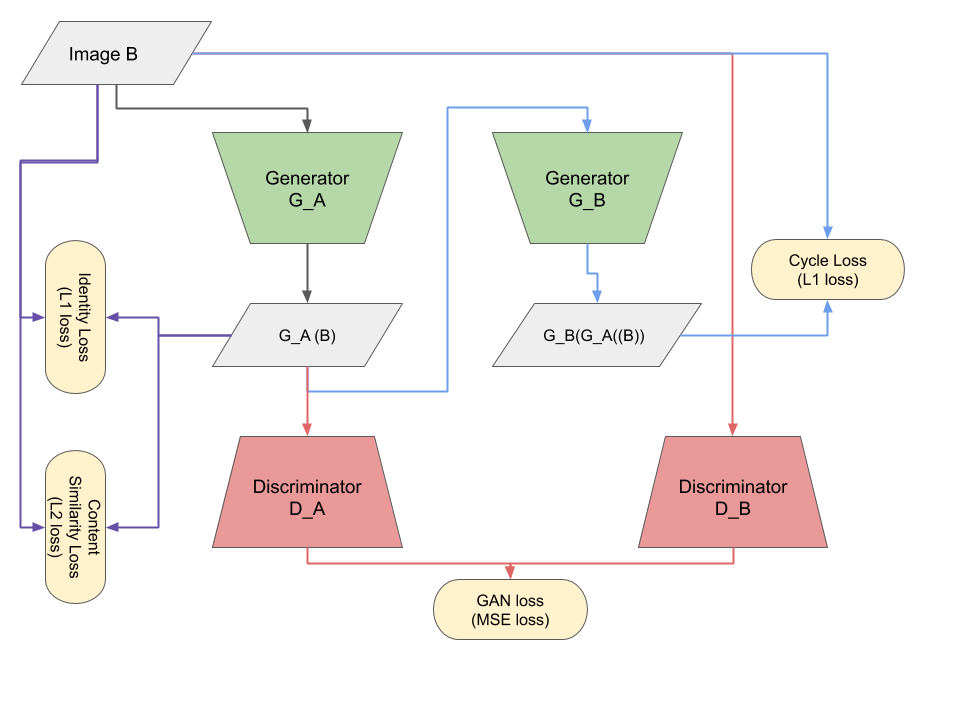
\includegraphics[width=0.99\linewidth]{ccg_model.png}
    \end{center}
   \caption{\textit{Model components and loss functions}. In this figure we
   just show components and pathways arising from input image from class B. The same things also exists for class A and have been omitted for the sake of simplicity.}
    \label{fig:model_and_loss}
\end{figure}

The generator architecture is 6 residual blocks sandwiched between two Convolution-InstanceNorm-ReLU layer. The discriminator has 4 Convolution-InstanceNorm-LeakyReLU layers. The content similarity block has a single Convolution-InstanceNorm-ReLU layer where the convolution weights are from a pretrained VGG-11 network and were not optimized for during the training.

\begin{figure}[tbp]
    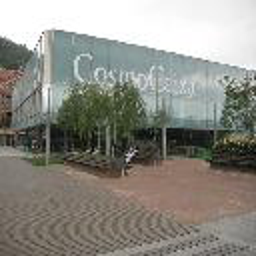
\includegraphics[width=.23\textwidth]{images/0002_real.png}\hfill
    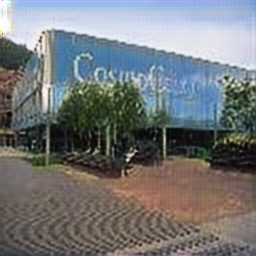
\includegraphics[width=.23\textwidth]{images/0002_fake.png}
    \\[\smallskipamount]
    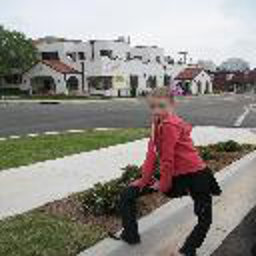
\includegraphics[width=.23\textwidth]{images/0018_real.png}\hfill
    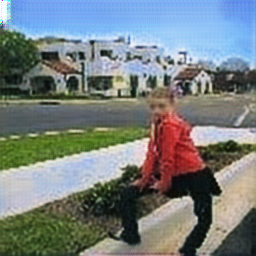
\includegraphics[width=.23\textwidth]{images/0018_fake.png}
    \\[\smallskipamount]
    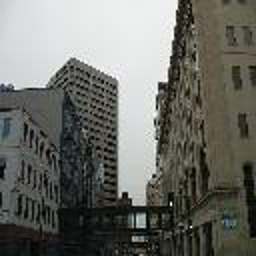
\includegraphics[width=.23\textwidth]{images/0027_real.png}\hfill
    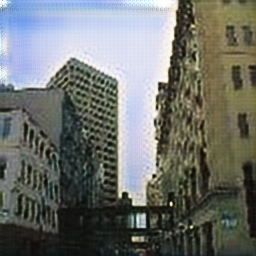
\includegraphics[width=.23\textwidth]{images/0027_fake.png}
    \caption{Sample results from the baseline model. The left column are cloudy input images and right column contains the corresponding generated sunny images.}\label{fig:og_model}
\end{figure}


\section{Experiments and Results}
As an initial baseline, we tried adapting the original Cycle-GAN model \cite{zhu2017unpaired} to this task. Rather than training it from scratch, we took the winter2summer model that was presented in the Cycle-GAN paper and trained it on our sunny/cloudy images. The reasoning behind this was that the tasks are similar in that they both are changing conditions of a given image. The content of the images is largely the same, but the colors and lighting represent a majority of the change. Training this for a couple epochs already posed some problems. Sample results are presented in Figure \ref{fig:og_model}. The models primarily focuses on making the sky blue, but it appears overdone fake. We can also notice the checkerboard artifacts, specially in the sky.

\begin{figure}[tpb]
    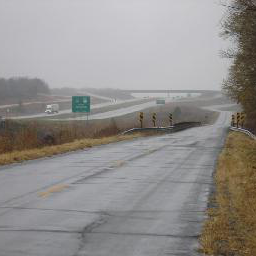
\includegraphics[width=.23\textwidth]{images/8_A.png}\hfill
    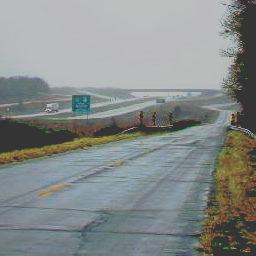
\includegraphics[width=.23\textwidth]{images/8_A2B.png}
    \\[\smallskipamount]
    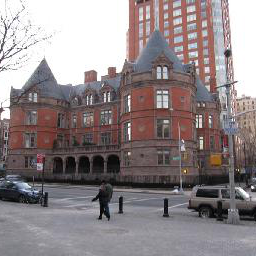
\includegraphics[width=.23\textwidth]{images/9_A.png}\hfill
    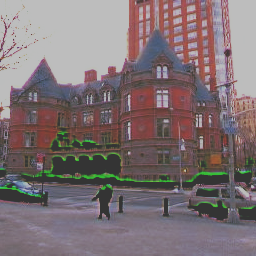
\includegraphics[width=.23\textwidth]{images/9_A2B.png}
    \caption{Results without the content similarity loss. Notice the blacked out regions and appearance of green artifacts }\label{fig:no_content_sim}
\end{figure}

\begin{figure*}[htpb]
  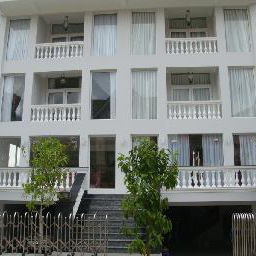
\includegraphics[width=.23\textwidth]{images/28_A.png} \hfill
  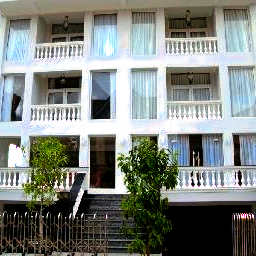
\includegraphics[width=.23\textwidth]{images/28_A2B.png} \hfill
  \hspace{1em}
  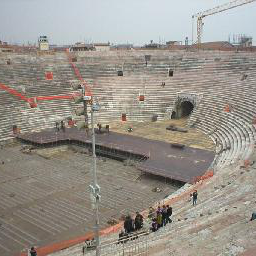
\includegraphics[width=.23\textwidth]{images/32_A.png} \hfill
  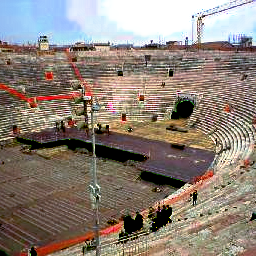
\includegraphics[width=.23\textwidth]{images/32_A2B.png} \hfill
  \\[\smallskipamount]
  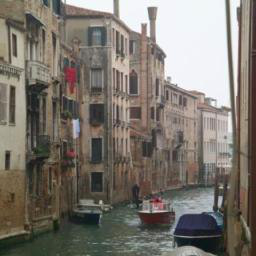
\includegraphics[width=.23\textwidth]{images/33_A.png} \hfill
  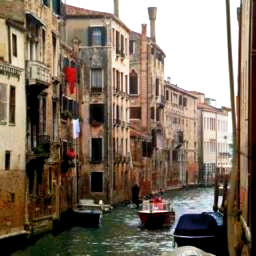
\includegraphics[width=.23\textwidth]{images/33_A2B.png} \hfill
  \hspace{1em}
  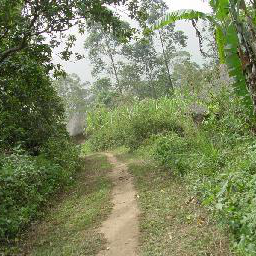
\includegraphics[width=.23\textwidth]{images/39_A.png} \hfill
  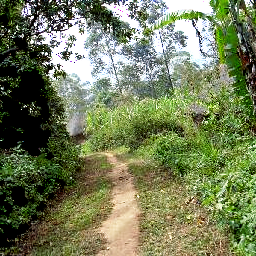
\includegraphics[width=.23\textwidth]{images/39_A2B.png} \hfill
  \\[\smallskipamount]
  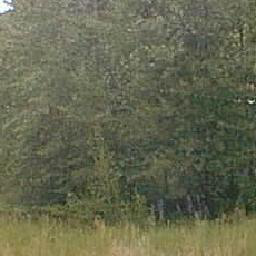
\includegraphics[width=.23\textwidth]{images/88_A.png} \hfill
  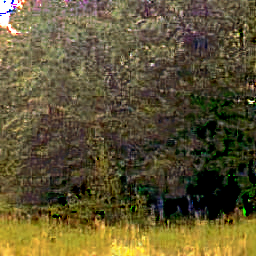
\includegraphics[width=.23\textwidth]{images/88_A2B.png} \hfill
  \hspace{1em}
  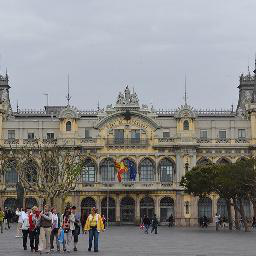
\includegraphics[width=.23\textwidth]{images/75_A.png}\hfill
  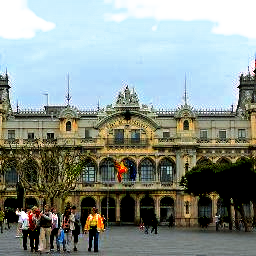
\includegraphics[width=.23\textwidth]{images/75_A2B.png}\hfill
  \\[\smallskipamount]
  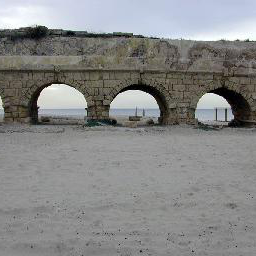
\includegraphics[width=.23\textwidth]{images/97_A.png}\hfill
  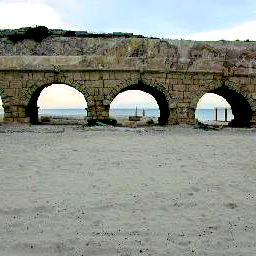
\includegraphics[width=.23\textwidth]{images/97_A2B.png}\hfill
  \hspace{1em}
  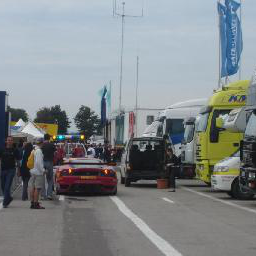
\includegraphics[width=.23\textwidth]{images/48_A.png}\hfill
  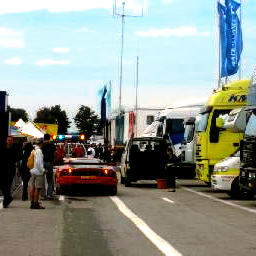
\includegraphics[width=.23\textwidth]{images/48_A2B.png}\hfill
  \caption{Final model results of cloudy to sunny translation. Column 1 and 3 are cloudy input images. Column 2 and 4 are corresponding output images images}\label{fig:results}
\end{figure*}
\begin{figure*}[htbp]
    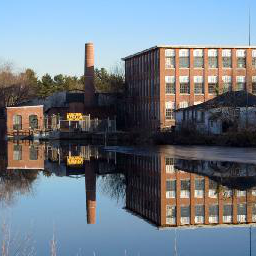
\includegraphics[width=.23\textwidth]{images/68_B.png}\hfill
  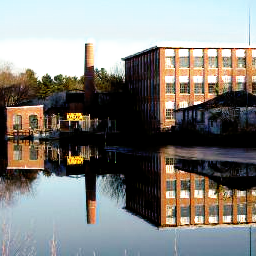
\includegraphics[width=.23\textwidth]{images/68_B2A.png}\hfill
  \hspace{1em}
  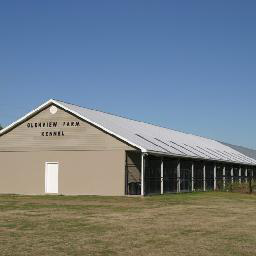
\includegraphics[width=.23\textwidth]{images/25_B.png}\hfill
  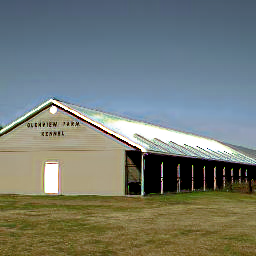
\includegraphics[width=.23\textwidth]{images/25_B2A.png}\hfill    
  \caption{Final model results of sunny to cloudy translation. Column 1 and 3 are sunny input images. Column 2 and 4 are corresponding output images }\label{fig:results2}
\end{figure*}


These artifacts and higher computation time for training prompted us to make the changes in the generator and discriminator architecture. Sample images are presented in Figure \ref{fig:no_content_sim}. The change solved the checkerboard pattern artifact but introduced weird artifacts. The grassy or very dark parts of the images on the left become blocked out in their sunny versions on the right. Entire parts of the brush are blocked off in this solid dark green color. We also see a bright green outline appearing on a number of objects. 

To address this, the Content Similarity Loss was introduced. We tried Alexnet first and then moved to VGG11 as it generated better results. Figures \ref{fig:results} and \ref{fig:results2} show some of the results from the final model.

The final model was trained using Adam over 100 epochs, starting with random weight initialization. This was based on \cite{zhu2017unpaired}, where the authors trained for 200 epochs for most of their tasks. This appears to a be a simpler problem than something like style transfer, so we chose 100. The learning rate started at 2e-4 and linearly decayed to 0 after 50 epochs. Training using the dataset took 8.5 hours in total, using a T4 GPU through Google Cloud. Figure \ref{fig:lossplot} shows the loss plots, with all the different losses broken down. 
\begin{figure}[htpb]
    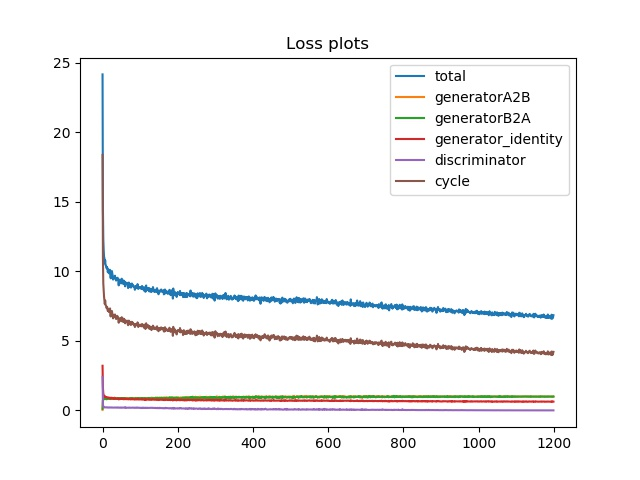
\includegraphics[width=.45\textwidth]{images/loss_plot.jpg}
    \caption{The loss plots during training over 100 epochs. The discriminator loss drops very quickly and is much smaller than the generator loss. }\label{fig:lossplot}
\end{figure}

The discriminator loss drops rapidly in comparison with the generator losses, effectively slowing down training. This is a reasonably common issue within GAN architectures, where the discriminator loss disappears, in a sense overpowering the generator. The discriminator is very good at telling the generated images from the real, so the generator continues to do poorly. Ideally, the loss should balance each other out in some fashion so learning can continue. When the discriminator loss goes to zero, generator stops getting better at sampling the images from the desired target distribution.

\subsection{Evaluation}
Densely connected convolutional network (DenseNet) was employed in comparing the performance of our cycle-GAN against a quantitative baseline. We chose the transfer learning approach in order to initialize the parameters from a network pre-trained on ImageNet data and modify the final fully connected layer of the pre-trained network to a new fully-connected layer producing 2 responses indicative of the predicted probabilities of the two classes(cloudy or sunny). We initially trained this image classification model on our source data-set and achieved a per class accuracy of 86\%. This model was later tested on an equal sized generated image dataset which resulted in a per class accuracy of 68\%. Figure \ref{fig:eval} gives us a summary of results obtained in evaluation of the two test datasets.
\begin{figure}[htbp]
    \begin{center}
        %\fbox{\rule{0pt}{2in} \rule{.9\linewidth}{0pt}}
        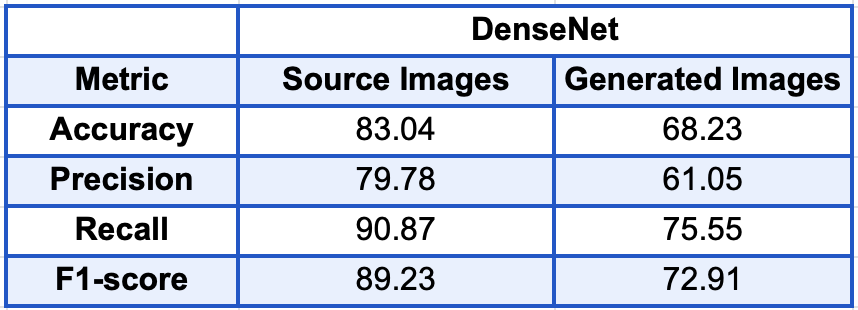
\includegraphics[width=0.9\linewidth]{images/Evaluation.png}
    \end{center}
   \caption{\textit{Summary of results obtained in the supervised binary classification task when tested on source images and generated images. }}
    \label{fig:eval}
\end{figure}

\section{Implementation details}
The dataset of cloudy and sunny images was downloaded from \cite{lu2014two}. It has 5000 images for each class. We divided the dataset into train, val, and test set using 70-15-15 split, resulting in 3500 images for training. The preprocessing applied was to center the dataset.

We implemented the model in \href{https://pytorch.org/}{Pytorch}. The authors of cycle-GAN have a public repository in Pytorch which we initially tried using their pre-trained models, which was trained on a different task. We then developed code for this project from scratch, using their code as a reference in some places. We had to redo the code as we introduced a new content similarity block, and changed the architecture to reduce the number of parameters to allow faster training.

The code is publicly available on Github at this \href{https://github.com/ayushbaid/cloudy-cycle-gans}{link}.

\section{Conclusion}
The cycle-GAN architecture with our modifications learns the color distribution of different components like sky, reflective surfaces, and the general contrast and brightness of the scene. However, the training time is too high. Also, the discriminator learns very quickly and does not generate gradients of sufficient magnitude for the generator, which stagnates the learning process. Different discriminator designs can be evaluated for this task which help overcome this problem.

{\small
\bibliographystyle{ieee}
\bibliography{egbib}
}

\end{document}
